\documentclass{ximera}
\input{../preamble.tex}

 \title{Linear Independence} \license{CC BY-NC-SA 4.0}

\begin{document}

\begin{abstract}
 \end{abstract}
\maketitle

\begin{onlineOnly}
\section*{Linear Independence}
\end{onlineOnly}

%\begin{summary}
%Let's review what we have learned in the previous three sections.  Let $\{\vec{v}_1, \vec{v}_2,\dots\,\vec{v}_n\}$ be a collection of vectors.  

%For scalars $a_1$, $a_2,\dots, a_n$, the expression $a_1\vec{v}_1+a_2\vec{v}_2+\dots +a_n\vec{v}_n$ is called \wordChoice{\choice[correct]{a linear combination} \choice{the sum}} of $\vec{v}_1, \vec{v}_2,\dots\,\vec{v}_n$.

%The set of all linear combinations of $\vec{v}_1, \vec{v}_2,\dots\,\vec{v}_n$ is called \wordChoice{\choice[correct]{the span} \choice{a linear combination} \choice{the sum}} of $\vec{v}_1, \vec{v}_2,\dots\,\vec{v}_n$.
%\end{summary}


In the last section  we considered properties a set of vectors should possess in order to be used to define a ``good'' coordinate system for a plane.  Let $S$ be a set of vectors in the plane.  We have already established that in order to use vectors in $S$ to define the axes of a ``good'' coordinate system, vectors in $S$ must span the plane.  This would guarantee that every vector in the plane can be written as a linear combination of elements of $S$.  

In addition, we observed that we want each vector in the plane to be represented as a \textit{unique} linear combination of elements of $S$.  This gives us motivation to consider the question of uniqueness.  We will now step away from coordinate systems in the plane and turn to this question in a more general setting.

Let $\vec{v}_1, \vec{v}_2,\dots ,\,\vec{v}_k$ be vectors of $\RR^n$.  Let $V=\text{span}(\vec{v}_1, \vec{v}_2,\dots ,\,\vec{v}_k)$.  Then every vector in $V$ can be written as a linear combination of $\vec{v}_1, \vec{v}_2,\dots ,\,\vec{v}_k$ in at least one way.  Our interest here is in spanning sets where each vector in $V$ has exactly one representation as a linear combination of $\vec{v}_1, \vec{v}_2,\dots ,\,\vec{v}_k$.

Suppose that two linear combinations are equal
 $$a_1\vec{v}_1+a_2\vec{v}_2+\dots +a_k\vec{v}_k=b_1\vec{v}_1+b_2\vec{v}_2+\dots +b_k\vec{v}_k$$ 
We are looking for a condition on the set $\{\vec{v}_1, \vec{v}_2,\dots ,\,\vec{v}_k\}$ that guarantees that this representation is unique.  This amounts to showing that $a_i=b_i$ for each $i$.  Taking all terms to the left side gives us
$$(a_1-b_1)\vec{v}_1+(a_2-b_2)\vec{v}_2+\dots +(a_k-b_k)\vec{v}_k=\vec{0}$$

So the condition that guarantees uniqueness is that all coefficients $(a_i-b_i)$ must be zero.  This motivates the following definition.

\begin{definition}[Linear Independence]\label{def:linearindependence}
Let $\vec{v}_1, \vec{v}_2,\ldots ,\vec{v}_k$ be vectors of $\RR^n$.  We say that the set $\{\vec{v}_1, \vec{v}_2,\ldots ,\vec{v}_k\}$ is \dfn{linearly independent} if the only solution to 
\begin{equation}\label{eq:defLinInd}c_1\vec{v}_1+c_2\vec{v}_2+\ldots +c_p\vec{v}_k=\vec{0}\end{equation}
is the \dfn{trivial solution} $c_1=c_2=\ldots =c_k=0$.

If, in addition to the trivial solution, any \dfn{non-trivial solutions} (not all $c_1, c_2,\ldots ,c_k$ are zero) exist, then we say that the set $\{\vec{v}_1, \vec{v}_2,\ldots ,\vec{v}_k\}$ is \dfn{linearly dependent}.
\end{definition}

\begin{observation}
The trivial solution $c_1=c_2=\ldots =c_k=0$ is always a solution to $c_1\vec{v}_1+c_2\vec{v}_2+\ldots +c_p\vec{v}_k=\vec{0}$ because $0\vec{v}_1+0\vec{v}_2+\ldots +0\vec{v}_k=\vec{0}$. So, when checking for linear independence, the question is not whether the trivial solution is a solution, but whether it is the ONLY solution.
\end{observation}

\begin{remark}\label{remark:LinIndEquiv}
Given a set of vectors $X=\{\vec{v}_1,\vec{v}_2,\dots,\vec{v}_k\}$ we can now ask the following questions:
\begin{enumerate}
\item Are the vectors in $X$ linearly dependent according to Definition \ref{def:linearindependence}?
\item Can we write one element of $X$ as a linear combination of the others?
    \item Does $X$ contain redundant vectors?
\end{enumerate}
It turns out that these questions are equivalent.  In other words, if the answer to one of them is ``YES", the answer to the other two is also ``YES".  Conversely, if the answer to one of them is ``NO", then the answer to the other two is also ``NO".  We will start by illustrating this idea with an example, then conclude this section by formally proving the equivalency in Theorem \ref{th:lindeplincombofother}.
\end{remark}

\begin{example}\label{ex:linind}What can we say about the following sets of vectors in light of Remark \ref{remark:LinIndEquiv}?

\begin{enumerate}
\item \label{item:linindpart1}
$$\left\{\begin{bmatrix}2\\-3\end{bmatrix}, \begin{bmatrix}0\\3\end{bmatrix},\begin{bmatrix}1\\-1\end{bmatrix},\begin{bmatrix}1\\-2\end{bmatrix}\right\}$$

\item \label{item:linindpart2} $$\left\{\begin{bmatrix}2\\1\\4\end{bmatrix},\begin{bmatrix}-3\\1\\1\end{bmatrix}\right\}$$
\end{enumerate}
\begin{explanation} \ref{item:linindpart1}
We will start by addressing linear independence.  To do so, we will solve the vector equation
\begin{align}\label{eq:linrelationpart1}c_1\begin{bmatrix}2\\-3\end{bmatrix}+c_2 \begin{bmatrix}0\\3\end{bmatrix}+c_3\begin{bmatrix}1\\-1\end{bmatrix}+c_4\begin{bmatrix}1\\-2\end{bmatrix}=\vec{0}\end{align}
 
 Clearly $c_1=c_2=c_3=c_4=0$ is a solution to the equation.  The question is whether another solution exists.
 
The vector equation translates into the following system:

$$\begin{array}{ccccccccc}
      2c_1 & &&+&c_3&+&c_4&= &0 \\
        -3c_1& +&3c_2&-&c_3&-&2c_4&= &0 \\
      \end{array}$$
  Writing the system in augmented matrix form and applying elementary row operations gives us the following reduced row-echelon form:
  $$\left[\begin{array}{cccc|c}  
 2&0&1&1&0\\-3&3&-1&-2&0
 \end{array}\right]\rightsquigarrow\left[\begin{array}{cccc|c}  
 1&0&1/2&1/2&0\\0&1&1/6&-1/6&0
 \end{array}\right]$$
 This shows that (\ref{eq:linrelationpart1}) has infinitely many solutions:  
 $$c_1=-\frac{1}{2}s-\frac{1}{2}t,\quad c_2=-\frac{1}{6}s+\frac{1}{6}t,\quad c_3=s,\quad c_4=t$$
 Letting $t=s=6$, we obtain the following:
 
 \begin{equation}\label{eq:ex1}
 -6\begin{bmatrix}2\\-3\end{bmatrix}+0 \begin{bmatrix}0\\3\end{bmatrix}+6\begin{bmatrix}1\\-1\end{bmatrix}+6\begin{bmatrix}1\\-2\end{bmatrix}=\vec{0}
 \end{equation}
 We conclude that the vectors are linearly dependent.

 Observe that (\ref{eq:ex1})  allows us to solve for one of the vectors and express it as a linear combination of the others. For example, 
\begin{equation}\label{eq:ex1lincomb}
    \begin{bmatrix}2\\-3\end{bmatrix}=0 \begin{bmatrix}0\\3\end{bmatrix}+\begin{bmatrix}1\\-1\end{bmatrix}+\begin{bmatrix}1\\-2\end{bmatrix}
\end{equation}
This would not be possible if a nontrivial solution to the equation
$$c_1\begin{bmatrix}2\\-3\end{bmatrix}+c_2 \begin{bmatrix}0\\3\end{bmatrix}+c_3\begin{bmatrix}1\\-1\end{bmatrix}+c_4\begin{bmatrix}1\\-2\end{bmatrix}=\vec{0}$$
did not exist.

Using the linear combination in (\ref{eq:ex1lincomb}) and the argument of Exploration \ref{exp:redundantVecs2}, we conclude that $\begin{bmatrix}2\\-3\end{bmatrix}$ is redundant in 
$$\left\{\begin{bmatrix}2\\-3\end{bmatrix}, \begin{bmatrix}0\\3\end{bmatrix},\begin{bmatrix}1\\-1\end{bmatrix},\begin{bmatrix}1\\-2\end{bmatrix}\right\}$$
We find that the answer to all questions in Remark \ref{remark:LinIndEquiv} is ``YES".
 
 
 \ref{item:linindpart2} To address linear independence, we need to solve the equation
 
 $$c_1\begin{bmatrix}2\\1\\4\end{bmatrix}+c_2\begin{bmatrix}-3\\1\\1\end{bmatrix}=\vec{0}$$
 Converting the equation to augmented matrix form and performing row reduction gives us
 $$\left[\begin{array}{cc|c}  
 2&-3&0\\1&1&0\\4&1&0
 \end{array}\right]\rightsquigarrow\left[\begin{array}{cc|c}  
 1&0&0\\0&1&0\\0&0&0
 \end{array}\right]$$
 This shows that $c_1=c_2=0$ is the only solution.  Therefore the two vectors are linearly independent.
 
 Furthermore, we cannot write one of the vectors as a linear combination of the other.  (Do you see that the only way this would be possible with a set of two vectors is if they were scalar multiples of each other?)
 
Finally, we observe that removing either vector would change the span from a plane in $\RR^3$ to a line in $\RR^3$, so the answer to all three questions in Remark \ref{remark:LinIndEquiv} is ``NO".
\end{explanation}
\end{example}

We now formalize Remark \ref{remark:LinIndEquiv} as a theorem.

\begin{theorem}\label{th:lindeplincombofother}
Let $\vec{v}_1,\vec{v}_2,\dots ,\vec{v}_k$ be  a set of vectors in $\RR^n$ containing two or more vectors.  The following conditions are equivalent.
\begin{enumerate}
\item\label{th:lindeplincombofother_a} 
%There exists a non-trivial solution to $c_1\vec{v}_1+c_2\vec{v}_2+\dots +c_k\vec{v}_k=\vec{0}$.
$\vec{v}_1,\vec{v}_2,\dots ,\vec{v}_k$ are linearly dependent.
\item\label{th:lindeplincombofother_b} 
One of $\vec{v}_1,\vec{v}_2,\dots ,\vec{v}_k$ can be expressed as a linear combination of the others.
\item\label{th:lindeplincombofother_c} 
The set $\{\vec{v}_1,\vec{v}_2,\dots ,\vec{v}_k\}$ contains redundant vectors.
\end{enumerate}
\end{theorem}

\begin{proof}
 \ref{th:lindeplincombofother_a} $\implies$ \ref{th:lindeplincombofother_b}  If $\vec{v}_1,\vec{v}_2,\dots ,\vec{v}_k$ are linearly dependent, then 
 \begin{equation*}c_1\vec{v}_1+c_2\vec{v}_2+\ldots +c_j\vec{v}_j+\ldots +c_k\vec{v}_k=\vec{0}\end{equation*}
 
 has a non-trivial solution.  In other words at least one of the constants, say $c_j$, does not equal zero.  This allows us to solve for $\vec{v}_j$:

\begin{align*}
-c_j\vec{v}_j&=c_1\vec{v}_1+c_2\vec{v}_2+\ldots +c_k\vec{v}_k \\ \\
\vec{v}_j&=-\frac{c_1}{c_j}\vec{v}_1-\frac{c_2}{c_j}\vec{v}_2-\ldots -\frac{c_k}{c_j}\vec{v}_k
\end{align*}
(Do you see why it was important to have one of the constants nonzero?)  This shows that $\vec{v}_j$ may be expressed as a linear combination of the other vectors.

\ref{th:lindeplincombofother_b} $\implies$ \ref{th:lindeplincombofother_c}  First, suppose $\vec{v}_j$ is a linear combination of $\vec{v}_1,\vec{v}_2,\dots,\vec{v}_k$.  We will show that $\vec{v}_j$ is redundant by showing that $$\mbox{span}\left(\vec{v}_1,\vec{v}_2,\dots,\vec{v}_k\right)=\mbox{span}\left(\vec{v}_1,\vec{v}_2,\dots,\vec{v}_{j-1},\vec{v}_{j+1},\dots,\vec{v}_k\right).$$
To show equality of the two spans we will pick a vector in the left span and show that it is also an element of the span on the right.  Then, we will pick a vector in the right span and show that it is also an element of the span on the left, and we will conclude that the sets are equal.

Observe that if $\vec{w}$ is in $\mbox{span}\left(\vec{v}_1,\vec{v}_2,\dots,\vec{v}_{j-1},\vec{v}_{j+1},\dots,\vec{v}_k\right)$, then it has to be in $\mbox{span}\left(\vec{v}_1,\vec{v}_2,\dots,\vec{v}_k\right)$. (Why?)

Now suppose $\vec{w}$ is in $\mbox{span}\left(\vec{v}_1,\vec{v}_2,\dots,\vec{v}_k\right)$.  We need to show that $\vec{w}$ is also in $\mbox{span}\left(\vec{v}_1,\vec{v}_2,\dots,\vec{v}_{j-1},\vec{v}_{j+1},\dots,\vec{v}_k\right)$.

By assumption, we can write $\vec{v}_j$ as
\begin{equation}\label{eq:vj}
\vec{v}_j=a_1\vec{v}_1+a_2\vec{v}_2+\dots +a_{j-1}\vec{v}_{j-1}+a_{j+1}\vec{v}_{j+1}+\dots +a_k\vec{v}_k.
\end{equation}

Since $\vec{w}$ is in $\mbox{span}\left(\vec{v}_1,\vec{v}_2,\dots,\vec{v}_k\right)$, we have
$$\vec{w}=b_1\vec{v}_1+b_2\vec{v}_2+\dots +b_j\vec{v}_j+\dots +b_k\vec{v}_k.$$
Substituting the expression in (\ref{eq:vj}) for $\vec{v}_j$ and simplifying, we obtain the following
\begin{eqnarray*}\vec{w}=(b_1+b_ja_1)\vec{v}_1+(b_2+b_ja_2)\vec{v}_2&+&\dots\\
&+&(b_{j-1}+b_ja_{j-1})\vec{v}_{j-1}\\
&+&(b_{j+1}+b_ja_{j+1})\vec{v}_{j+1}\\
&+&\dots\\
&+&(b_k+b_ja_k)\vec{v}_k.\end{eqnarray*}
This shows that $\vec{w}$ is in $\mbox{span}\left(\vec{v}_1,\vec{v}_2,\dots,\vec{v}_{j-1},\vec{v}_{j+1},\dots,\vec{v}_k\right)$.
We now have 
$$\mbox{span}\left(\vec{v}_1,\vec{v}_2,\dots,\vec{v}_k\right)=\mbox{span}\left(\vec{v}_1,\vec{v}_2,\dots,\vec{v}_{j-1},\vec{v}_{j+1},\dots,\vec{v}_k\right),$$
which shows that $\vec{v}_j$ is redundant.

 \ref{th:lindeplincombofother_c} $\implies$ \ref{th:lindeplincombofother_a}  Suppose that $\vec{v}_j$ is redundant, so that
 $$\mbox{span}\left(\vec{v}_1,\vec{v}_2,\dots,\vec{v}_k\right)=\mbox{span}\left(\vec{v}_1,\vec{v}_2,\dots,\vec{v}_{j-1},\vec{v}_{j+1},\dots,\vec{v}_k\right).$$
 Consider a vector $\vec{w}$ in $\mbox{span}\left(\vec{v}_1,\vec{v}_2,\dots,\vec{v}_k\right)$  
\begin{equation}\label{eq:w1}
\vec{w}=a_1\vec{v}_1+a_2\vec{v}_2+\dots +a_j\vec{v}_j+\dots +a_k\vec{v}_k
\end{equation}
Since the span contains ALL possible linear combinations of $\vec{v}_1,\vec{v}_2,\dots,\vec{v}_k$, we may choose $\vec{w}$ such that $a_j\neq 0$.

By assumption, $\vec{w}$ is also in $\mbox{span}\left(\vec{v}_1,\vec{v}_2,\dots,\vec{v}_{j-1},\vec{v}_{j+1},\dots,\vec{v}_k\right)$.  Therefore, we can express $\vec{w}$ as a linear combination 
\begin{equation}\label{eq:w2}
\vec{w}=b_1\vec{v}_1+b_2\vec{v}_2+\dots +b_{j-1}\vec{v}_{j-1}+b_{j+1}\vec{v}_{j+1}+\dots +b_k\vec{v}_k.
\end{equation}

 We complete the proof by showing there exists a non-trivial solution to 
\begin{equation}\label{eq:LinIndepDefRepeated}
c_1\vec{v}_1+c_2\vec{v}_2+\ldots +c_j\vec{v}_j+\ldots +c_k\vec{v}_k=\vec{0}.\end{equation}  Subtracting expression (\ref{eq:w2}) from (\ref{eq:w1}) we obtain
\begin{eqnarray*}
    \vec{0}=\vec{w}-\vec{w}=(a_1-b_1)\vec{v}_1&+&\dots\\ \nonumber
    &+&(a_{j-1}-b_{j-1})\vec{v}_{j-1}+a_j\vec{v}_j+(a_{j+1}-b_{j+1})\vec{v}_{j+1}\\ \nonumber
  &+&\dots\\ \nonumber
  &+&(a_k-b_k)\vec{v}_k
\end{eqnarray*}
Recall that we ensured that $a_j\neq 0$.  This implies that we have a non-trivial solution to Equation \ref{eq:LinIndepDefRepeated}.

These three parts of the proof show that if one of the conditions is true, all three must be true.  It is a logical consequence that if one of the three conditions is false, all three must be false.
 \end{proof}
 
\subsection*{Geometry of Linearly Dependent and Linearly Independent Vectors}

Theorem \ref{th:lindeplincombofother} gives us a convenient ways of looking at linear dependence/independence geometrically.  When looking at two or more vectors, we ask, ``can one of the vectors be written as a linear combination of the others?"  We can also ask, ``is one of the vectors redundant?''  If the answer to either of these questions is ``YES", then the vectors are linearly dependent.
\subsubsection*{A Set of Two Vectors}
Two vectors are linearly dependent if and only if one is a scalar multiple of the other.  Two nonzero linearly dependent vectors may look like this:
\begin{center}
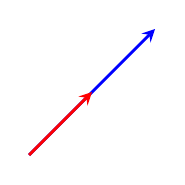
\begin{tikzpicture}[scale=0.8]
% \draw[<->] (-0.5,0)--(2.5,0);
 % \draw[<->] (0,-0.5)--(0,2.5);
    \draw[line width=1pt,blue,-stealth](0,0)--(2,2);
  \draw[line width=1pt,red,-stealth](0,0)--(1,1);
 \end{tikzpicture}
\end{center}
or like this:
\begin{center}
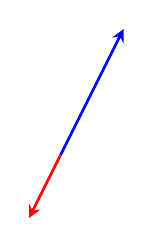
\begin{tikzpicture}[scale=0.8]
%\draw[<->] (-2.5,0)--(2.5,0);
 % \draw[<->] (0,-2.5)--(0,2.5);
    \draw[line width=1pt,blue,-stealth](0,0)--(1,2);
  \draw[line width=1pt,red,-stealth](0,0)--(-0.5,-1);
 \end{tikzpicture}
\end{center}
Two linearly independent vectors will look like this:
\begin{center}
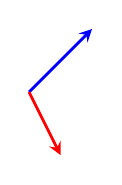
\begin{tikzpicture}[scale=0.8]
%\draw[<->] (-2.5,0)--(2.5,0);
 % \draw[<->] (0,-2.5)--(0,2.5);
    \draw[line width=1pt,blue,-stealth](0,0)--(1,1);
  \draw[line width=1pt,red,-stealth](0,0)--(0.5,-1);
 \end{tikzpicture}
\end{center}
\subsubsection*{A Set of Three Vectors}
Given a set of three nonzero vectors, we have the following possibilities: 
\begin{itemize}
\item (Linearly Dependent Vectors)
The three vectors are scalar multiples of each other.
\begin{center}
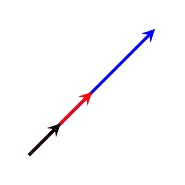
\begin{tikzpicture}[scale=0.8]
% \draw[<->] (-0.5,0)--(2.5,0);
 % \draw[<->] (0,-0.5)--(0,2.5);
    \draw[line width=1pt,blue,-stealth](0,0)--(2,2);
  \draw[line width=1pt,red,-stealth](0,0)--(1,1);
  \draw[line width=1pt,-stealth](0,0)--(0.5,0.5);
 \end{tikzpicture}
\end{center}
\item (Linearly Dependent Vectors) Two of the vectors are scalar multiples of each other.
\begin{center}
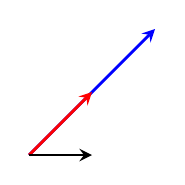
\begin{tikzpicture}[scale=0.8]
    \draw[line width=1pt,blue,-stealth](0,0)--(2,2);
  \draw[line width=1pt,red,-stealth](0,0)--(1,1);
  \draw[line width=1pt,-stealth](0,0)--(1,0);
 \end{tikzpicture}
\end{center}
\item (Linearly Dependent Vectors) One vector can be viewed as the diagonal of a parallelogram determined by scalar multiples of the other two vectors.  All three vectors lie in the same plane.
\begin{center}
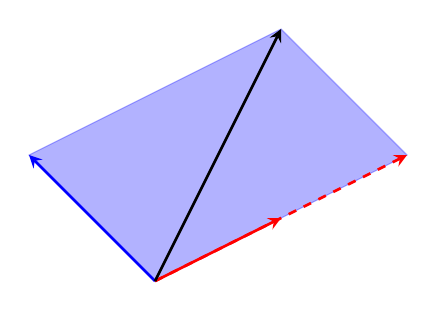
\begin{tikzpicture}[scale=0.8]
  \filldraw[blue, opacity=0.3](0,0)--(-2,2)--(2,4)--(4,2)--cycle;
\draw[line width=1pt,red,-stealth](0,0)--(2,1);
\draw[line width=1pt,red,-stealth, dashed](0,0)--(4,2);
  \draw[line width=1pt,blue,-stealth](0,0)--(-2,2);
  \draw[line width=1pt,-stealth](0,0)--(2,4); 
\end{tikzpicture}
\end{center}
\item (Linearly Independent Vectors)
A set of three vectors is linearly independent if the vectors do not lie in the same plane.  For example, vectors $\vec{i}$, $\vec{j}$ and $\vec{k}$ are linearly independent.
\end{itemize}

\section*{Practice Problems}



 \begin{problem}\label{prob:linindmultchoice1}
 Are the vectors below linearly independent?
$$\begin{bmatrix}-1\\0\end{bmatrix}, \begin{bmatrix}2\\3\end{bmatrix},\begin{bmatrix}4\\-1\end{bmatrix}$$

\begin{multipleChoice}
 \choice{Yes}
  \choice[correct]{No }
 \end{multipleChoice}
 \begin{hint}
 If we rewrite $$c_1\begin{bmatrix}-1\\0\end{bmatrix}+c_2 \begin{bmatrix}2\\3\end{bmatrix}+c_3\begin{bmatrix}4\\-1\end{bmatrix}=\begin{bmatrix}0\\0\end{bmatrix}$$ as a system of linear equations, there will be more unknowns than equations.
 \end{hint}
\end{problem}

\begin{problem}\label{prob:linindmultchoice2}
 Are the vectors below linearly independent?
$$\begin{bmatrix}1\\0\\5\end{bmatrix}, \begin{bmatrix}2\\2\\3\end{bmatrix},\begin{bmatrix}-1\\0\\1\end{bmatrix}$$

\begin{multipleChoice}
 \choice[correct]{Yes}
  \choice{No }
 \end{multipleChoice}
\begin{hint}
If we let $A$ be the matrix whose columns are these vectors, then $\mbox{rref}(A)$ should tell us what we want to know.
\end{hint}
\end{problem}

\begin{problem}\label{prob:linindmultchoice3}
 Are the vectors below linearly independent?
$$\begin{bmatrix}3\\0\\5\end{bmatrix}, \begin{bmatrix}2\\0\\2\end{bmatrix},\begin{bmatrix}-1\\0\\-5\end{bmatrix}$$

\begin{multipleChoice}
 \choice{Yes}
  \choice[correct]{No }
 \end{multipleChoice}
 \begin{hint}
 If we let $A$ be the matrix whose columns are these vectors, then $\mbox{rref}(A)$ should tell us what we want to know.
 \end{hint}
\end{problem}

\begin{problem}\label{prob:linindmultchoice4}
 Are the vectors below linearly independent?
$$\begin{bmatrix}3\\1\\4\\1\end{bmatrix}, \begin{bmatrix}-2\\1\\1\\1\end{bmatrix}$$

\begin{multipleChoice}
 \choice[correct]{Yes}
  \choice{No }
 \end{multipleChoice}
 \begin{hint}
 In a set of two vectors, the only way one could be redundant is if they are scalar multiples of each other.
 \end{hint}

\end{problem}

\begin{problem}\label{prob:TFlinind1}
(True or False?) Any set containing the zero vector is linearly dependent.
\begin{multipleChoice}
 \choice[correct]{TRUE}
  \choice{FALSE}
 \end{multipleChoice}
  \begin{hint}
 Can the zero vector be removed from the set without changing the span?
 \end{hint}
 \end{problem}
 
\begin{problem}\label{prob:TFlinind2}
(True or False?) A set containing five vectors in $\RR^2$ is linearly dependent.
\begin{multipleChoice}
 \choice[correct]{TRUE}
  \choice{FALSE}
 \end{multipleChoice}
  \begin{hint}
 If we rewrite Equation \ref{eq:defLinInd} for five vectors in $\RR^2$ as a system of equations, how many equations and unknowns will it have?  What does this imply about the number of solutions?
 \end{hint}
\end{problem}


\begin{problem}\label{prob:linindmultchoice5}
Given that
$$0\vec{v}_1+ 0\vec{v}_2+ 0\vec{v}_3=\vec{0}$$
what (if anything) can we conclude about linear independence of vectors $\vec{v}_1, \vec{v}_2, \vec{v}_3$?
\begin{multipleChoice}
 \choice{The vectors are linearly independent}
  \choice{The vectors are linearly dependent }
  \choice[correct]{There is not enough information given to make a determination }
 \end{multipleChoice}
\end{problem}

\begin{problem}\label{prob:linindmultchoice6}
Given that
$$3\vec{v}_1+ 4\vec{v}_2- \vec{v}_3=\vec{0}$$
what (if anything) can we conclude about linear independence of vectors $\vec{v}_1, \vec{v}_2, \vec{v}_3$?
\begin{multipleChoice}
 \choice{The vectors are linearly independent}
  \choice[correct]{The vectors are linearly dependent }
  \choice{There is not enough information given to make a determination }
 \end{multipleChoice}
\end{problem}

\begin{problem}\label{prob:linindmultchoice7}
Given that
$$2\vec{v}_1+ 0\vec{v}_2+ 0\vec{v}_3=\vec{0}$$
what (if anything) can we conclude about linear independence of vectors $\vec{v}_1, \vec{v}_2, \vec{v}_3$?
\begin{multipleChoice}
 \choice{The vectors are linearly independent}
  \choice[correct]{The vectors are linearly dependent }
  \choice{There is not enough information given to make a determination }
 \end{multipleChoice}
\end{problem}



\begin{problem}\label{prob:linindmultchoice9}
Are the vectors in the diagram linearly dependent or independent?
\begin{multipleChoice}
 \choice{The vectors are linearly independent}
  \choice[correct]{The vectors are linearly dependent }
  \choice{There is not enough information given to make a determination }
 \end{multipleChoice}
\begin{center}
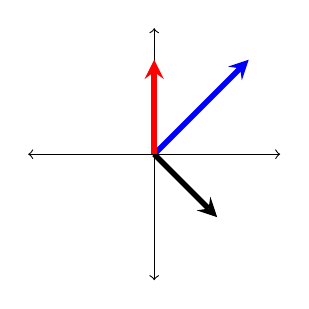
\begin{tikzpicture}[scale=0.8]
  \draw[<->] (-2,0)--(2,0);
  \draw[<->] (0,-2)--(0,2);
  
  \draw[line width=2pt,blue,-stealth](0,0)--(1.5,1.5);
  \draw[line width=2pt,-stealth](0,0)--(1,-1);
  \draw[line width=2pt,red,-stealth](0,0)--(0,1.5);

 \end{tikzpicture}
\end{center}
\end{problem}

\begin{problem}\label{prob:linindmultchoice10}
Are the vectors in the diagram linearly dependent or independent?
\begin{multipleChoice}
 \choice[correct]{The vectors are linearly independent}
  \choice{The vectors are linearly dependent }
  \choice{There is not enough information given to make a determination }
 \end{multipleChoice}
\begin{center}
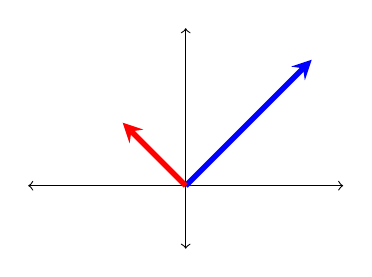
\begin{tikzpicture}[scale=0.8]
  \draw[<->] (-2.5,0)--(2.5,0);
  \draw[<->] (0,-1)--(0,2.5);
  
  \draw[line width=2pt,blue,-stealth](0,0)--(2,2);
  \draw[line width=2pt,red,-stealth](0,0)--(-1,1);

 \end{tikzpicture}
\end{center}
\end{problem}


\begin{problem}\label{prob:Adding1OK}
Suppose $\{\vec{v}_{1}, \dots , \vec{v}_{m}\}$ is a linearly independent set in $\RR^n$, and that $\vec{v}_{m+1}$ is not in $\mbox{span}\left(\vec{v}_{1}, \dots , \vec{v}_{m}\right)$.  Prove that $\{\vec{v}_{1}, \dots , \vec{v}_{m}, \vec{v}_{m+1}\}$ is also linearly independent.
\end{problem}

\begin{problem}\label{prob:OtherLinearComb}
Suppose $\{{\vec{u}},{\vec{v}}\}$ is a linearly independent set of vectors.  Prove that the set $\{\vec{u} -\vec{v}, \vec{u}+2\vec{v}\}$ is also linearly independent.
\end{problem}

\begin{problem}\label{prob:OtherLinearComb2}
Suppose $\{{\vec{u}},{\vec{v}}\}$ is a linearly independent set of vectors in $\RR^3$.  Is the following set dependent or independent $\{\vec{u} -\vec{v}, \vec{u}+2\vec{v}, \vec{u}+\vec{v}\}$? Prove your claim.
\end{problem}

\section*{Text Source} A portion of this section was adapted from Section 5.2 of Keith Nicholson's \href{https://open.umn.edu/opentextbooks/textbooks/linear-algebra-with-applications}{\it Linear Algebra with Applications}. (CC-BY-NC-SA)
 
W. Keith Nicholson, {\it Linear Algebra with Applications}, Lyryx 2018, Open Edition, p. 271.
\end{document} 